% This is based on LLNCS.dem the demonstration file of
% the LaTeX macro package from Springer-Verlag
% for Lecture Notes in Computer Science,
% version 2.4 for LaTeX2e as of 16. April 2010
%
% Modified by Gabriele Bleser, January 2013
% Modified by Oliver Wasenmüller, March 2016
% Modified by Oliver Wasenmüller, November 2017
% 
% This is the Latex main document. If you need additional packages, 
% you can insert them here. Otherwise you should not modify this.
% Provide your contribution in a separate file, such as mypaper.tex.
% All contributions will be included here.
%

\documentclass{llncs}

% Include your packages here
\usepackage{graphicx}
\usepackage{textcomp}
\usepackage{listings}
\usepackage{subfiles}
\usepackage{subfigure}
\usepackage{amsmath}
\usepackage{url}
\usepackage{bm}
%\usepackage[german]{babel}

% use this for revew submission only. Please comment it for final submission
%\usepackage{lineno}
%\linenumbers
%

\begin{document}

\pagestyle{headings}  % switches on printing of running heads

%
\title{Seamless Cloth Simulation with High Geometric Fidelity}
%
\titlerunning{Cloth Simulation}  % abbreviated title (for running head)
%
\author{Sikang Yan\inst{1} \and Sk Aziz Ali\inst{2} \and Wolfgang Dornisch\inst{3}}
%
\authorrunning{Yan et al.} % abbreviated author list (for running head)
%
\institute{\email{yan@rhrk.uni-kl.de}
\and
\email{Sk$\_$Aziz.Ali@dfki.uni-kl.de}
\and
\email{dornisch@rhrk.uni-kl.de}}

\maketitle              % typeset the title of the contribution

\begin{abstract}
Despite a large volume of studies, a current particle dynamic system results plausible deformation of draping, folding, wrinkling, stretching, etc., but realistic fold patterns generated from body-pose based variations and motion ill pose the problem. In this paper, a new approach based on continuum mechanic is proposed, which     
\keywords{keyword1, keyword2, }
\end{abstract}


% This is your content. Name the sections appropriately
\section{Introduction}

\section{}
\subsection{Deformation Gradient}
Let $\kappa$ be a reference configuration and $\Gamma$ be an arbitrary configuration of body $\mathcal{B}$. Then the mapping 
 \begin{align}
  \mathbf{x}=\Gamma_{\kappa}( \mathbf{X},t ) 
 \end{align}
is called the \emph{deformation} of body $\mathcal{B}$ from $\kappa$ to $\Gamma$.

The \emph{deformation gradient} $\mathbf{F}$ of $\Gamma$ relative to $\kappa$, is defined by
 \begin{align}
  \mathbf{F}= \nabla_{\mathbf{X}} \Gamma_{\kappa} = \dfrac{\partial \mathbf{x}}{\partial \mathbf{X}}
  =
  \renewcommand\arraystretch{2}
  \begin{bmatrix}
    \dfrac{\partial x}{\partial X} & \dfrac{\partial x}{\partial Y} & \dfrac{\partial x}{\partial Z}  \\
    \dfrac{\partial y}{\partial X} & \dfrac{\partial y}{\partial Y} & \dfrac{\partial y}{\partial Z}  \\
    \dfrac{\partial z}{\partial X} & \dfrac{\partial z}{\partial Y} & \dfrac{\partial z}{\partial Z}  \\ 
  \end{bmatrix},  
 \label{eq:deformation_gradient} 
 \end{align}
where the coordinates of $\mathbf{X}$ are called the \emph{template coordinates} and the coordinates of $\mathbf{x}$ are called the \emph{reference coordinates}. Moreover, the Eq. \eqref{eq:deformation_gradient} is a measure of local deformation of the body. Hence the mapping $\Gamma_{\kappa}$ is one-to-one and onto, $\mathbf{F}$ is non-singular. 

Applied by \emph{decomposition theorem} on the deformation gradient \cite{liu2002continuum}, there exist two positive definite symmetric tensor $\mathbf{U}$ and $\mathbf{V}$, and an orthogonal tensor $\mathbf{R}$, uniquely determined by $\mathbf{F}$, such that 
\begin{align}
\mathbf{F}=\mathbf{R}\mathbf{U}=\mathbf{V}\mathbf{R},
\label{eq:decomposition_theorem}
\end{align}
where the $\mathbf{U}$ and $\mathbf{V}$ denote the \emph{right} and \emph{left stretch tensor}, and $\mathbf{R}$ denotes the local \emph{rotation tensor}. As a consequence of Eq. \eqref{eq:decomposition_theorem}, we could obtain the pure stretches by applying
 \begin{align}
  \mathbf{U}^2=\mathbf{F}^T\mathbf{F}=\mathbf{C} \quad \mbox{and} \quad \mathbf{V}^2=\mathbf{F}\mathbf{F}^T=\mathbf{B},
  \label{eq:stretch_tensor}
 \end{align} 
where the $\mathbf{C}$ and $\mathbf{B}$ are called \emph{right} and \emph{left Cauchy-Green strain tensor}.

Since $\mathbf{C}$ can be diagonalized as 
\begin{align}
\mathbf{C} =  \lambda_1^2 \mathbf{e}_1 \mathbf{e}_1^T+ \lambda_2^2 \mathbf{e}_2 \mathbf{e}_2^T+ \lambda_3^2 \mathbf{e}_3 \mathbf{e}_3^T,
\end{align}
we could calculated the $\mathbf{U}$ by applying 
\begin{align}
\mathbf{U} =  \lambda_1 \mathbf{e}_1 \mathbf{e}_1^T+ \lambda_2 \mathbf{e}_2 \mathbf{e}_2+ \lambda_3 \mathbf{e}_3 \mathbf{e}_3^T.
\label{eq:strech_tensor_diagonalized}
\end{align}
The $\lambda_1<\lambda_2<\lambda_3$ are real, positive eigenvalues and the corresponding $\mathbf{e_1},\mathbf{e_2},\mathbf{e_3}$ are unit eigenvectors, defining main stretch or shrinkage directions \cite{wriggers2013nichtlineare}.

Following by \cite{rohmer2010animation}, the \emph{wrinkle vector field} $\mathbf{v}$ describes the rate of shrinkage per unit of length wherever shrinkage occurs and its direction is orthogonal to the
main shrinkage direction, which is given by
\begin{align}
\mathbf{v}=\max (1-\lambda_1,0) \mathbf{e}_2.
\end{align}

\subsection{Velocity Gradient}
Whereas the deformation gradient measures the local deformation, the \emph{spacial velocity gradient} $\mathbf{L}$ describes the rate of deformation, given by
\begin{align}
\mathbf{L} = grad \bm{v} = \dot{\mathbf{F}} \mathbf{F}^{-1},
\end{align}
where $\bm{v}$ denotes the \emph{velocity} of the material point $\mathbf{X}$, and $\dot{\mathbf{F}}$ denotes the material time derivative of deformation gradient $\mathbf{F}$. 

Analogically, we apply the polar decomposition on the spacial velocity gradient $\mathbf{L}$\cite{liu2002continuum}, and obtain
\begin{align}
\mathbf{L} = \mathbf{D}+\mathbf{W}.
\end{align}
Thus, the tensor $\mathbf{L}$ could be decomposed into its symmetric part $\mathbf{D}$ and skew-symmetric part $\mathbf{W}$
\begin{align}
\mathbf{D}=&\dfrac{1}{2}(\mathbf{L}+\mathbf{L}^T), \\
\mathbf{W}=&\dfrac{1}{2}(\mathbf{L}-\mathbf{L}^T).
\end{align}
where $\mathbf{D}$ is called the \emph{rate of strain tensor}, and $\mathbf{W}$ is called the \emph{rate of rotation tensor}.

Assuming $\rm{d}\mathbf{x}$ is a material line element in the current configuration, the rate of change of its length $\dot{\epsilon}_{ii}$ and angle $\dot{\gamma}_{ij}$ is measured by means of $\mathbf{D}$\cite{haupt2013continuum}.
\begin{align}
\dot{\epsilon}_{ii}=&\mathbf{e}_i\mathbf{D}\mathbf{e}_i=D_{ii} \\
\dot{\gamma}_{ij}=&2\mathbf{e}_i\mathbf{D}\mathbf{e}_j=D_{ij}
\end{align}
where $D_{ij}$ are the $ij$-entries of $\mathbf{D}$. Additionally, if $\mathbf{D}$ has the same base ${\mathbf{e_1},\mathbf{e_2},\mathbf{e_3}}$ as in the eq.\eqref{eq:strech_tensor_diagonalized}, then
\begin{align}
D_{11}=&\dfrac{\dot{\lambda_1}}{\lambda_1} \\
D_{22}=&\dfrac{\dot{\lambda_2}}{\lambda_3} \\
D_{33}=&\dfrac{\dot{\lambda_2}}{\lambda_3} 
\end{align}

Given the deformation gradients at the beginning $F_t$ and end $F_{t+\Delta t}$ of a time step, we use \emph{forward difference} \cite{wilmott1995mathematics} to calculate the derivation of deformation gradient and take the inverse of the later one.  

\subsection{Cross-covariance Matrix}
Let $\Phi$ denote the points set in the template frame, and $\Psi$ denote the points set in the reference frame. Therefore, each set of points can be described as
\begin{align}
\Phi=
  \begin{bmatrix}
    X_1 & Y_1 & Z_1  \\
    X_2 & Y_2 & Z_2  \\
    \vdots & \vdots & \vdots \\
    X_N & Y_N & Z_N 
  \end{bmatrix}
\quad \mbox{and} \quad
\Psi=
  \begin{bmatrix}
    x_1 & y_1 & z_1  \\
    x_2 & y_2 & z_2  \\
    \vdots & \vdots & \vdots \\
    x_N & y_N & z_N 
  \end{bmatrix},
\end{align}
where $N$ is the number of the points in the points set.

A point $\overline{\mathbf{j}}$ is called the \emph{neighboring point} of point $\mathbf{j}$, when $\overline{\mathbf{j}}$ and $\mathbf{j}$ are connected by a same edge. If only the data set without any further information is given, we shall use the \emph{kd-tree} \cite{bentley1975multidimensional} as a data structure to search for the neighboring points in no structural points set. 

Let $\overline{\Phi} \subset \Phi$ define the points set of the neighboring points of $\mathbf{X}_i$ in the template frame, and $\overline{\Psi} \subset \Psi$ define the points set of the neighboring points of $\mathbf{x}_i$ in the reference frame. Therefore, we could construct a $M \times 3$ matrix $\mathbf{P}_i$ for each point $\mathbf{X}_i \in \Phi$, as well as a matrix $\mathbf{Q}_i$ for each point $\mathbf{x}_i \in \Psi$,
\begin{align}
\mathbf{P}_i=
  \begin{bmatrix}
    X_1-X_i & Y_1-Y_i & Z_1-Z_i  \\
    X_2-X_i & Y_2-Y_i & Z_2-Z_i  \\
    \vdots & \vdots & \vdots \\
    X_M-X_i & Y_M-Y_i & Z_M-Z_i 
  \end{bmatrix} 
\quad \mbox{and} \quad 
 \mathbf{Q}_i=
  \begin{bmatrix}
    x_1-x_i & y_1-y_i & z_1-z_i  \\
    x_2-x_i & y_2-y_i & z_2-z_i  \\
    \vdots & \vdots & \vdots \\
    x_M-x_i & y_M-y_i & z_M-z_i  \\
  \end{bmatrix},
\end{align}
where $\mathbf{X}_1,\mathbf{X}_2,\dots,\mathbf{X}_M \in \overline{\Phi}$ and $\mathbf{x}_1,\mathbf{x}_2,\dots,\mathbf{x}_M \in \overline{\Psi}$, and $M$ is the number of the points in the neighboring points set. The matrices $\mathbf{P}_i$ and $\mathbf{Q}_i$ represent the distribution of local shapes near the point $\mathbf{X}_i$ and $\mathbf{x}_i$, see Fig. \ref{fig:neighboring_point}.
\begin{figure}
 \centering
 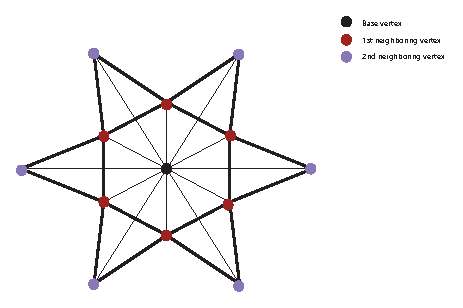
\includegraphics[width=0.5\textwidth]{image//neighboring_point.eps}
 \caption{The neighboring vertices of one base vertex in a structural points set.}
 \label{fig:neighboring_point}
\end{figure}  

Proceeding to define
\begin{align}
\mathbf{H} = \mathbf{P}^T \mathbf{Q}.
\end{align}
$\mathbf{H}$ is called the \emph{cross-covariance matrix}, which is a measure of similarity of $\mathbf{P}$ and $\mathbf{Q}$ \cite{park2017fundamentals}. 

The matrix $\mathbf{H}$ is derived from the \emph{orthogonal Procrustes problem}\cite{schonemann1966generalized}. It is defined as the least-squares problem of transforming a given matrix $\mathbf{P}$ into a given matrix $\mathbf{Q}$ by an orthogonal transformation matrix $\mathbf{R}$, such that the sums of squares of the residual matrix $\mathbf{E}=\mathbf{\Omega} \mathbf{P} - \mathbf{Q}$ is a minimum
\begin{align}
\mathbf{R}=\mathop{\arg\min}_{\mathbf{\Omega}} \| \mathbf{\Omega} \mathbf{P} - \mathbf{Q} \|_{F} \quad \mbox{subject to} \quad \mathbf{\Omega}^T\mathbf{\Omega}=\mathbf{I},
\end{align}
where $\| \cdot \|_{F}$ is the Frobenius norm. Moreover, it can be shown\cite{zhang2000flexible} that this problem is equivalent to find the nearest orthogonal matrix $\mathbf{R}$ to a given matrix $\mathbf{H} = \mathbf{P}^T \mathbf{Q}$, which most closely maps $\mathbf{P}$ to $\mathbf{Q}$. Thus, we could use $\mathbf{H}$ to approximate the deformation gradient $\mathbf{F}$ in Eq. \eqref{eq:deformation_gradient}
\begin{align}
\widetilde{\mathbf{F}} = \mathbf{H}.
\end{align}

Applied by Eq. \eqref{eq:decomposition_theorem} \eqref{eq:stretch_tensor} \eqref{eq:strech_tensor_diagonalized}, we could obtain the approximated stretch tensor $\widetilde{\mathbf{U}}$ and its eigenvalues $\tilde{\lambda_1},\tilde{\lambda_2},\tilde{\lambda_3}$.

\section{Animation of Wrinkle Deformation Field}
\subsection{Structural Points Sets Using 1st Neighboring Points}


\subsection{Structural Points Sets Using 2nd Neighboring Points}

\subsection{Non-structural Points Sets Using Binary Search Tree}


\section{Conclusion}


%

%
% ---- Bibliography ----
%
\bibliographystyle{plain}
\bibliography{llncs}
%
\end{document}
